\documentclass[a4paper,12pt,fleqn]{article}
\usepackage{amsmath, amssymb}
\usepackage{bbm}
\usepackage{enumitem}
\usepackage{array}
\usepackage{fancyhdr}
\usepackage{graphicx}

% Insert your course information here %%%%%%%%%%%%%%%%%%%%%%%%%%%%%%%%%%

\newcommand{\titlehd}{Computational Data Analysis}
\newcommand{\examtype}{\bf Final Exam}
\newcommand{\examdate}{Due Dec. 13, 2019}
\newcommand{\examcode}{ISYE 6740}
%\newcommand{\writetime}{}
\newcommand{\total}{100}
\newcommand{\lastwords}{End of Examination}

%%%%%%%%%%%%%%%%%%%%%%%%%%%%%%%%%%%%%%%%%%%%%%%%%%%%

%\setcounter{MaxMatrixCols}{10}
\newtheorem{theorem}{Theorem}
\newtheorem{acknowledgement}[theorem]{Acknowledgement}
\newtheorem{algorithm}[theorem]{Algorithm}
\newtheorem{axiom}[theorem]{Axiom}
\newtheorem{case}[theorem]{Case}
\newtheorem{claim}[theorem]{Claim}
\newtheorem{conclusion}[theorem]{Conclusion}
\newtheorem{condition}[theorem]{Condition}
\newtheorem{conjecture}[theorem]{Conjecture}
\newtheorem{corollary}[theorem]{Corollary}
\newtheorem{criterion}[theorem]{Criterion}
\newtheorem{definition}[theorem]{Definition}
\newtheorem{example}[theorem]{Example}
\newtheorem{exercise}[theorem]{Exercise}
\newtheorem{lemma}[theorem]{Lemma}
\newtheorem{notation}[theorem]{Notation}
\newtheorem{problem}[theorem]{Problem}
\newtheorem{proposition}[theorem]{Proposition}
\newtheorem{remark}[theorem]{Remark}
\newtheorem{solution}[theorem]{Solution}
\newtheorem{summary}[theorem]{Summary}
\newenvironment{proof}[1][Proof]{\noindent\textbf{#1.} }{\ \rule{0.5em}{0.5em}}
\newcounter{questionnumber}
\stepcounter{questionnumber}

\newcommand{\questionnumber}{\noindent \arabic{questionnumber}\stepcounter{questionnumber})~~}
\newcommand{\truefalse}[1]{\questionnumber #1\\True~~~~~~~~False\\Explanation if False:\\ \vspace{3cm}}
\newcommand{\norm}[1]{\|#1\|}
\newcommand{\RR}{\mathbb{R}}
\newcommand{\argmin}{\mathop{\arg\min}}

% ANU Exams Office mandated margins and footer style
\setlength{\topmargin}{0cm}
\setlength{\textheight}{9.25in}
\setlength{\oddsidemargin}{0.0in}
\setlength{\evensidemargin}{0.0in}
\setlength{\textwidth}{16cm}
\pagestyle{fancy}
\lhead{} 
\chead{} 
\rhead{} 
\lfoot{} 
\cfoot{\footnotesize{Page \thepage \ of \pageref{finalpage} -- \titlehd \ (\examcode)}} 
\rfoot{} 

% DEPRECATED: ANU Exams Office mandated margins and footer style
%\setlength{\topmargin}{0cm}
%\setlength{\textheight}{9.25in}
%\setlength{\oddsidemargin}{0.0in}
%\setlength{\evensidemargin}{0.0in}
%\setlength{\textwidth}{16cm}
%\pagestyle{fancy}
%\lhead{} %left of the header
%\chead{} %center of the header
%\rhead{} %right of the header
%\lfoot{} %left of the footer
%\cfoot{} %center of the footer
%\rfoot{Page \ \thepage \ of \ \pageref{finalpage} \\
%       \texttt{\examcode}} %Print the page number in the right footer

\renewcommand{\headrulewidth}{0pt} %Do not print a rule below the header
\renewcommand{\footrulewidth}{0pt}


\begin{document}

% Title page
\begin{center}
\large\textbf{\titlehd}
\end{center}

\begin{center}
\large\textbf{\examcode}
\end{center}

\begin{center}
\textit{ \examtype -- \examdate}
\end{center}

%\begin{center}
%\textit{Writing Time: \writetime}
%\end{center}

\begin{center}
\textit{Total Score: \total}
\end{center}

\vspace{2cm}
If you think a question is unclear or multiple answers are reasonable, please write a brief explanation of your answer,
 to be safe. Also, show your work if you want wrong answers to have a chance at some credit: it lets us see how much you understood.\\\\
(Please sign the honor code below.) I have neither given nor received any unauthorized aid on this exam. I understand that the work contained herein is wholly my own without the aim from a 3rd person. I understand that violation of these rules, including using an authorized aid or copying from another person,
may result in my receiving a 0 on this exam .
\begin{table}[h]
\centering
\begin{tabular}{m{8cm}}
\\
\\
\vspace{0.2in}
\textbf{Name}: 
\vspace{0.7in}

\textbf{GT ID:}
\vspace{0.7in}


\textbf{GT Account:}
\end{tabular}
\end{table}
\newpage

\begin{table}[h]
\centering
\begin{tabular}{| m{6cm} | m{6cm} |}
\hline
\vspace{0.5cm}
Question 1 [15 points] & \\
\vspace{0.5cm} &\vspace{0.5cm}\\
\hline
\vspace{0.5cm}
Question 2 [15 points] & \\
\vspace{0.5cm} &\vspace{0.5cm}\\
\hline
\vspace{0.5cm}
Question 3 [15 points] & \\
\vspace{0.5cm} &\vspace{0.5cm}\\
\hline
\vspace{0.5cm}
Question 4 [20 points] &  \\
\vspace{0.5cm} &\vspace{0.5cm}\\
\hline
\vspace{0.5cm}
Question 5 [10 points] & \\
\vspace{0.5cm} &\vspace{0.5cm}\\\hline
\vspace{0.5cm}
Question 6 [25 points] & \\
\vspace{0.5cm} &\vspace{0.5cm}\\\hline

\hline
\end{tabular}
\end{table}


% End title page

%
%\newpage
%
%\section{K-means}
%\questionnumber{
%
%Given data points $x_1,x_2,\ldots,x_n \in \mathbb{R}^d$. We can modify K-means objective with $\ell_1$ regularization. More specifically, we consider
%\[
%\argmin_{S=\{S_1,\ldots,S_k\}} \sum_{j=1}^{k}\sum_{x_i\in S_j}\|x_i-\mu_j\|^2_2 + \lambda \sum_{j=1}^{k}\|\mu_j\|_1
%\]
%where $\lambda > 0$ is the regularization parameter.
%where $\mu_j$ is the mean of points in $S_j$. 
%
%\begin{enumerate}
%	
%	\item[(a)]  Please describe the new 2-steps optimization for this problem. Are they different from the original problem?
%	
%	(Hint: you may need the fact that,$$\hat v = \argmin_v \frac{1}{2}\|u-v\|^2_2+\lambda \|v\|_1$$ has closed form solution $\hat{v}  = [\hat{v}_j]_{j=1}^d = [\mathrm{sign}(u_j)\max\{|u_j|-\lambda,0\}_{j=1}^d].$)
%	
%	\vspace*{160pt}
%	
%	\item[(b)] The $\ell_1$ regularization encourages sparsity of $\mu_j$ . If the results have the $m$-th entries of all $\mu_j$'s equal to zero, what will this imply?
%	\vspace*{80pt}
%	
%	\item[(c)] Let $\gamma_k$ and $\gamma'_k$ denote the global optimal objective value of k-means with and without $\ell_1$ regularization. Please compare $\gamma_k$ and $\gamma'_k$ ($<,\leq,\geq,=$) and prove this relation.
%	\vspace*{80pt}
%\end{enumerate}
%
%}
%
%\newpage
%
%\section*{Question 2. Spectral Clustering}
%Recall that spectral clustering is a method finding $K$ clusters on a graph/network $\mathcal{G}=(\mathcal{V},\mathcal{E})$, where $\mathcal{V} = \{1,\ldots,n\}$ is the $\mathcal{E}$ is the edge set. $w_{ij}$ is the weight of edge $e=(i,j) \in \mathcal{E} $. A cluster is a subset of vertexes, i.e. $\mathcal{G}_k \subseteq \mathcal{V},\; k=1,\ldots,K$. We define two useful quantities on two subsets of vertexes, $A$ and $B$: 
%\[cut(A,B)=\sum_{i\in A,j\in B}w_{ij}
%\quad \text{and} \quad
%assoc(A) = cut(A,\mathcal{V})=\sum_{i\in A,j\in \mathcal{V}}w_{ij}
%\]
%Thus we can define cut cost function to evaluate the quality of clustering, $$R^C(\mathcal{G}_1,\ldots,\mathcal{G}_K)=\sum_{k=1}^{K}cut(\mathcal{G}_k,\mathcal{V} \backslash \mathcal{G}_k)$$
% and the normalized cut cost function
% $$R^{NC}(\mathcal{G}_1,\ldots,\mathcal{G}_K)=\sum_{k=1}^{K}\frac{cut(\mathcal{G}_k,\mathcal{V} \backslash \mathcal{G}_k)}{assoc(\mathcal{G}_k)}$$
% 
% \begin{enumerate}
% 	
% 	\item[(a)]  Please explain the intuition behind $cut(A,B),assoc(A),R^C,R^{NC}$
% 	
% 	
% 	\newpage
% 	For simplicity, in the following questions we only consider $K=2$
% 	
%% 	\item[(b)] Show that minimizing $R^{NC}(\mathcal{G}_1, \mathcal{G}_2)$ has the following formulation:
%% 	$$ \min R^{C}(\mathcal{G}_1, \mathcal{G}_2) = \min f^TLf , \quad 
%% 	\text{where}\ f_i=  
%% 	\left\{ \begin{aligned}
%% 	1, i\in \mathcal{G}_1\\
%% 	-1, i\in \mathcal{G}_2
%% 	\end{aligned}
%% 	\right.
%% 	$$
%% 	Recall that the graph Laplacians was defined as $L=D-W$, where $$D=diag(\sum_{j=1}^{n}w_{1j},\sum_{j=1}^{n}w_{2j},\ldots,\sum_{j=1}^{n}w_{nj})$$
%% 	
%% 	\item[(c)] We can we consider the relaxation of the above problem, i.e.,
%% 	 $$\min R^{C}(\mathcal{G}_1, \mathcal{G}_2) = \min f^TLf, \quad \text{subject to} \quad f^\top f = 1,$$ where the constraint is used to control the scale of $f$. Show that the solution of such problem is the eigen vector we used in the 
% 	
% 	\item[(b)] Show that minimizing $R^{NC}(\mathcal{G}_1, \mathcal{G}_2)$ has the following formulation:
% 	\begin{align} \min R^{NC}(\mathcal{G}_1, \mathcal{G}_2) = \min \frac{f^TLf}{f^TDf} , \quad 
% 	\text{where}\ f_i=  
% 	\left\{ \begin{aligned}
% 	\frac{1}{assoc(\mathcal{G}_1)}, i\in \mathcal{G}_1\\
% 	-\frac{1}{assoc(\mathcal{G}_2)}, i\in \mathcal{G}_2
% 	\end{aligned}
% 	\right. \label{eq:2.b}
% 	\end{align}
% 	Recall that the graph Laplacians was defined as $L=D-W$, where $$D=diag(\sum_{j=1}^{n}w_{1j},\sum_{j=1}^{n}w_{2j},\ldots,\sum_{j=1}^{n}w_{nj})$$
% 	
% 	\newpage
% 	\item[(c)] Next we consider the relaxation of the above problem, i.e.,
% 	\begin{align}\min R^{NC}(\mathcal{G}_1, \mathcal{G}_2) = \min \frac{f^TLf}{f^TDf}, \quad \text{subject to} \quad f^\top D\mathbf{1} = 0,\label{eq:2.c}
% 	\end{align}
% 	 Jusitify this is a relaxation of \eqref{eq:2.b}, i.e. for any solution of \eqref{eq:2.b} is a solution of \eqref{eq:2.c}
% 	
% 	\newpage
% 	\item[(d)] Show that the solution to \eqref{eq:2.c} is the eigen vector corresponding to second smallest eignevalue of the Graph Laplacian $L$. Just like the one we used in Spectral Clustering. (Noticing that the smallest eigenvalue is 0, and the corresponding eigen vector is $\mathbf{1}$) Here we can normalize $f$ for simplicity, i.e., you only need to consider the following problem
% 	 \begin{align}\min R^{NC}(\mathcal{G}_1, \mathcal{G}_2) = \min \frac{f^TLf}{f^TDf}=\min f^TLf, \notag \\ \text{subject to} \quad f^\top D\mathbf{1} = 0,\; f^TDf=1,\label{eq:2.d}
% 	\end{align} 
% 	where the additional constraint is only used for controlling the scale of $f$.
% 	\newpage
% 	
% \end{enumerate}

\clearpage
\section{Clustering [15 pts]}


\begin{enumerate}

\item (5 points) Explain what is the difference between $K$-means and spectral clustering? 
\vspace{.15in}

Both K-means and spectral clustering are able to programmatically assign data points into groups given a similarity/dissimilarity function.  The main difference between the two algorithms is that K-means, the much simpler algorithm, only uses a distance metric as it's similarity/dissimilarity measure. Spectral clustering, on the other hand, is able to use the geometry/connectivity of the data to assign data into groups. 

 
K-means steps:
\begin{enumerate}[label=(\roman*)]
\item  Initialize cluster centers
There are multiple ways to do this, either pick randomly within the feature space or pick a random K actual points from the dataset.

\item Assign each point to the closest cluster center 
\item Adjust the cluster centers based on the average center of the above assignment.
\item Iterate until cluster centers converge

\end{enumerate}

Spectral Clustering steps:
\begin{enumerate}[label=(\roman*)]
\item Build an adjacency matrix A using nearest neighbors
\item Represent graph as adjacency matrix $A \epsilon R^{mxm}$
\item Form a special matrix $L=D-A$ the graph Laplacian
\item Compute k eigenvectors of L corresponding to the k smallest eigenvalues
\item Run k-means algorithm on the above eigenbectors treating each row as a new datapoint
\end{enumerate}

The two methods above both use K-means as the end method to assign points into groups.  Spectral clustering has an initial data transformation that allows the final K-means operation to consider the connectivity of the data.
\vspace{.15in}



\item (5 points) What is in common, and what is the main difference between spectral clustering and PCA?

\vspace{.15in}
Spectral clustering and PCA are two methods that use eigendecomposition to find patterns within a dataset.  The difference between the two are how eigendecomposition is used within the algoritms.  

PCA uses eigendecomposition for dimensionality reduction.  The purpose is to preserve as much information of the underlying data as possible but reducing the dimensions to be able to visualize the data, apply simpler models to the data, or speed up a subsequent learning task.  After eigendecomposition, the eigenvectors that correspond to the K largest eigenvalues are chosen to represent the data.  The eigenvalues represent the variation in the data and variation can be seen as a proxy for information within the data.  It is therefore possible to drastically reduce the dimensions within while preserving the majority of the underlying information.  

Spectral clustering uses eigendecomposition to determine the connectedness of a graph.  It does this by  first finding the graph Laplacian of the data and then performing eigendecomposition on the transformed data.  

Both spectral clustering and PCA use eigendecomposition.  Data that has been transformed through PCA can be used for clustering, although the main goal is dimensionality reduction where spectral clustering is obviously used for clustering.

\vspace{.15in}

\item (5 points) For the following data (two moons), give one method that will successfully separate the two moons? Explain your rationale. 
\vspace{.15in}
Spectral clustering will be able to easily separate the below data.  K-means is not a viable option because it will only consider the distance between points not the connectedness of the data points.  The obvious separation of the points is the two moons, therefore spectral clustering's ability to consider the geometry of the data is the obvious choice to cluster the below data.  There will be a considerable eigengap between the 2 k smallest eigenvalues that will be able to determine the connectedness between the datapoints that make up each half moon.

\begin{center}
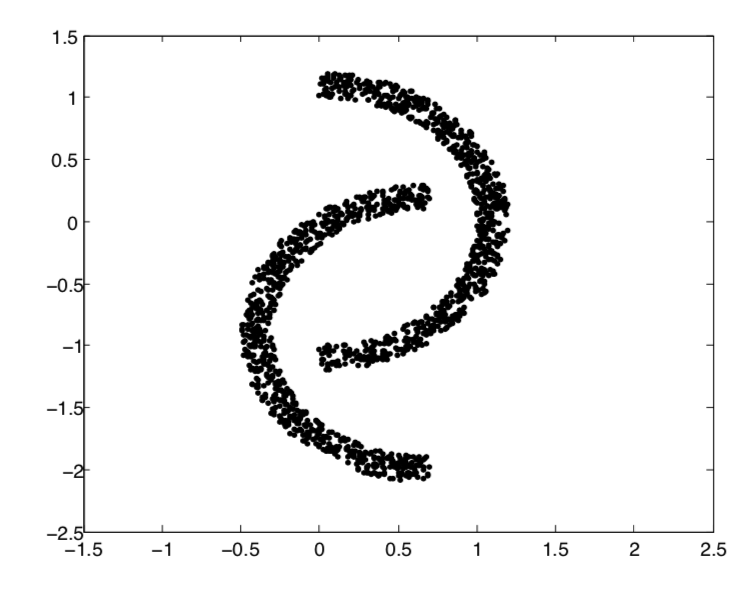
\includegraphics[width = 0.5\textwidth]{moon}
\end{center}

\end{enumerate}

\clearpage
\section{Classification [15 points]}

\begin{enumerate}
\item (5 points) List all methods below which can be used for classification:

(a) AdaBoost (b) Decision Trees (c) EM and Gaussian Mixture (d) Histogram (e) $K$-nearest neighbors (f) $K$-means (g) Kernel density estimation 
(h) Linear Regression (i) Logistic Regression (j) Naive Bayes. 



\vspace{.15in}
Methods that can be used for classification are:
\begin{itemize}
\item Adaboost
\item Decision Trees
\item EM and Gaussian Mixture Model
\item K-nearest neighbors
\item K-means (classification through clustering)
\item Logistic Regression
\item Naive Bayes

\end{itemize}
Kernel density estimation and histograms are not necessarily classification.  They can be used to determine the likelihood of a particular data point and are often used as a building block for more sophisticated classification algorithms.
\vspace{.15in}



\item (5 points) Which of the decision boundaries below correspond to (a) Random Forest, (b) Decision Tree, (c) SVM. Explain your reasons  to fully justify your answers. 

\vspace{.15in}

Going from left to right the decision boundaries correspond to SVM, decision tree, and random forest.

The first image is obviously SVM because the decision boundaries are linear and SVM is a linear classifier.  The next two decision boundaries are similar, but the last image on the very right performed better ($.85 > .78$) and looks like it has a lot more noise assoicated with it.  That extra noise and layers is the result of the randomness in the random forest, which generally performs better than the single decision tree.

%
\begin{center}
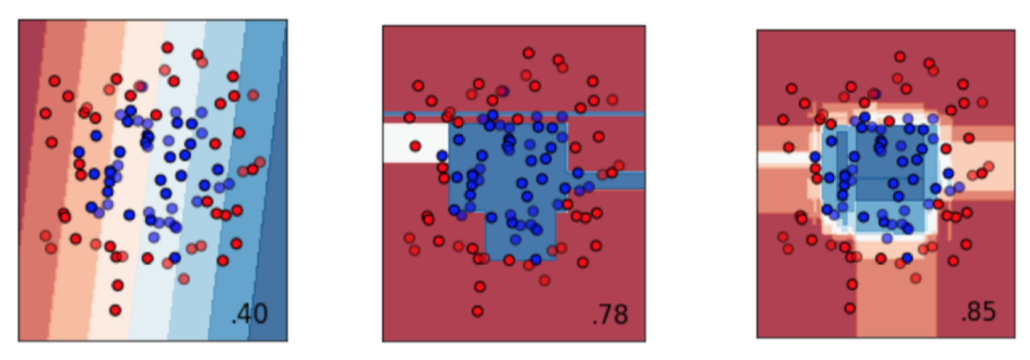
\includegraphics[width = 0.6\textwidth]{decision}
\end{center}

\vspace{.15in}

\item (5 points) Is the following statement true / false: ``In the AdaBoost algorithm, the weights on all the
misclassified points will go up by the same multiplicative factor.'' Explain your reason.

\vspace{.15in}
True, this comes from the equation used in updating, $D_T$.  All misclassified points are scaled equally in this equation to determine the new weights.
\vspace{.15in}

\end{enumerate}


\clearpage
\section{SVM [15 points]}

Suppose we only have four training examples in two dimensions as shown in Fig. The positive samples at $x_1 = (0, 0)$, $x_2 = (2, 2)$ and negative samples at $x_3 = (h, 1)$ and $x_4 = (0, 3)$. 
%
\begin{center}
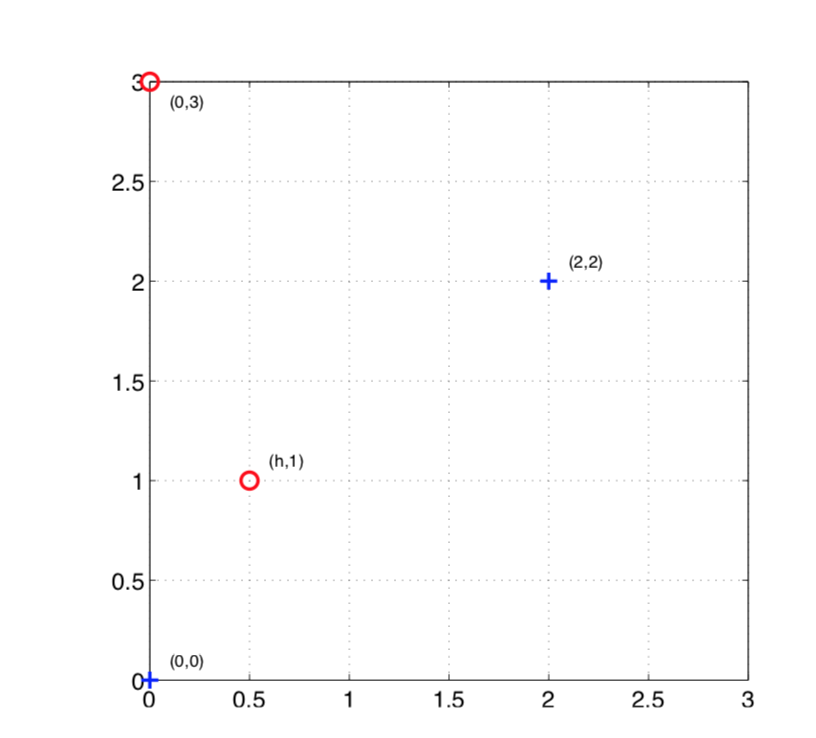
\includegraphics[width = 0.5\textwidth]{svm}
\end{center}

\begin{enumerate}
\item (5 points) For what $h$ s.t. $h > 0$ to be so that the training points are still linearly separable?

\vspace{.15in}
The blue cross class are on the line $y=x$ and the point in question has a $y=1$.  Therefore any $0 < h < 1$ should allow the points to be linearly sperable.
\vspace{.15in}

\item (5 points) Does the orientation of the maximum margin decision boundary change as a function of $h$ when the points are separable?

\vspace{.15in}
No because the other points remain and would be the support vecotrs.  
\vspace{.15in}

\item (5 points) Explain why only the data points on the ``margin'' will contribute to the decision boundary?
\end{enumerate}

\vspace{.15in}
The maximum margin decision boundary is the perpendicular distance between the margins of the decision boundary, so by definition they define the decision boundary.
\vspace{.15in}

\clearpage

\section{Variable section [20 points]}

Suppose we have data $\{x_i, y_i\}$, $i = 1, \ldots, m$, where $x_i \in \mathbb R^p$ corresponds to $p$ features.


\begin{enumerate}
\item (5 points) Write down the optimization problem we solve with Ridge Regression and Lasso. Make sure you explain your notations: which are the decision variables, and which are data. 

\vspace{.15in}
Ridge Regression:

Given $m$ data points, find $\theta$ that minimizes the regularized mean square error.  Where $x$ are the features and y are the target variables, $\theta$ is the decision variable to be optimized and $\lambda$ a positive regularization paramter that can be tuned.

$$
\theta^r = argmin_{\theta}L(\theta) = \frac{1}{m}\sum_{i=1}^{m} (y^i -\theta^Tx^i)^2+\lambda||\theta||^2
$$



\vspace{.15in}
Lasso Regression:

Given $m$ data points, find $\theta$ that minimizes the regularized mean square error.  Where $x$ are the features and y are the target variables, $\theta$ is the decision variable to be optimized and $\lambda$ a positive regularization paramter that can be tuned.


$$
\hat{\theta} = argmin_{\theta}L(\theta) = \frac{1}{m}\sum_{i}^{m} (y^i -\theta^Tx^i)^2+\lambda||\theta||
$$

\vspace{.15in}

\item (5 points) Which of the solution paths below corresponds to Ridge regression and which corresponds to Lasso?
%
\begin{center}
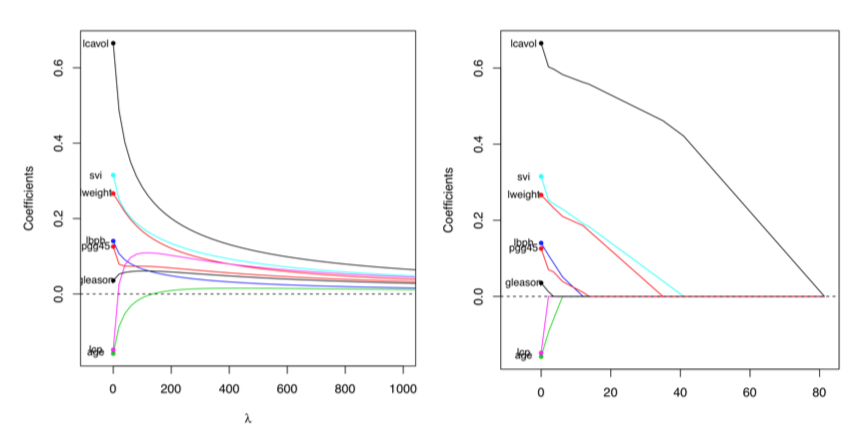
\includegraphics[width = 0.6\textwidth]{path}
\end{center}

\vspace{0.15in}
Ridge regression force coefficients to be lower, but it does not force them to 0.  Lasso can actually return 0 coefficients.  Therefore the left hand image is Ridge and the right is Lasso.

\vspace{0.15in}
\item (5 points) Explain what's the difference between Lasso and Ridge regression. We need Lasso for what setting?

\vspace{0.15in}
The difference between Ridge and Lasso are the regularization terms.  Lasso uses L1 regularization and Ridge uses L2 regularization.  L1 regularization, as discussed above is able to set coefficients to 0.  This has the added benefit of a built in feature selection tool.  


\vspace{0.15in}

\item (5 points) Explain how to tune the regularization parameters for Lasso and Ridge regression. 

\vspace{.15in}
Cross validation is used to tune the regularization parameter $\lambda$.  K-fold cross-validation is performed by the steps below.


For each fold $i$:
\begin{enumerate}[label=\arabic*)]
\item set aside $\alpha \cdot m$ samples of $D$ (where $m = |D|$) as the held-out data.  They will be used to evaluate the error.
\item Fit a model to the remaining $(1-\alpha)\cdot m$ samples in $D$
\item Calculate the error of the model with the held-out data.
\end{enumerate}
\vspace{.15in}

Repeat the above K times, choosing a different held-out data set each time, and the errors are averaged over the folds.  

K-fold cross-validation is performed on different values of $\lambda$ and the $\lambda$ that results in the lowest error is chosen.
 

\end{enumerate}


\clearpage

\section{Neural networks [10 points].}

\begin{enumerate}
\item (5 points)
Consider a neural networks for a binary classification using sigmoid function for each unit. If the network has no hidden layer, explain why the model is equivalent to logistic regression. 

\vspace{.15in}
A neural network is basically a combination of layered and stacked generalized linear models, which logistic regression is a member of.  If you have just a single perceptron, without any hidden layers, and choose the logit as your activation function, this is equivalent to logistic regression.

\vspace{.15in}


\item (5 points) 
Consider a simple two-layer network in the lecture slides. Given $m$ training data $(x^i, y^i)$, $i = 1, \ldots, m$, the cost function used to training the neural networks
\[
\ell(w, \alpha, \beta) = \sum_{i=1}^m (y^i - \sigma(w^T z^i))^2
\]
where $\sigma (x) = 1/(1+e^{-x})$ is the sigmoid function, $z^i$ is a two-dimensional vector such that  $z_1^i = \sigma(\alpha^T x^i)$, and $z_2^i = \sigma(\beta^T x^i)$. Show the that the gradient is given by
\[
\frac{\partial \ell(w, \alpha, \beta) }{\partial w}
= \sum_{i=1}^m 2(y^i - \sigma(u^i))\sigma(u^i)(1-\sigma(u^i)) z^i,
\]
where $u^i = w^T z^i$. Also find the gradient of $\ell(w, \alpha, \beta)$ with respect to $\alpha$ and $\beta$ and write down their expression.
\end{enumerate}
\vspace{.15in}

\vspace{.15in}
\clearpage

\section{Programming: Bayes and KNN classifier [25 points]}


In this programming assignment, you are going to apply the Bayes Classifier to handwritten digits classification problem. Here, we use the binary 0/1 loss for binary classification, i.e., you will calculate the miss-classification rate as a performance metric.

To ease your implementation, we selected two categories from USPS dataset in \textsf{usps-2cls.mat} (or \textsf{usps-2cls.dat}, \textsf{usps-2cls.csv}).

\begin{enumerate}
\item (15 points)
Your first task is implementing the classifier by assuming the covariance matrices for two classes are a diagonal matrix $\Sigma_1$, $\Sigma_ 2$. 

Using slides from ``Classification I'', assuming $P(y=1) = P(y=-1)$ (i.e., the prior distribution for two classes are the same), using Bayes decision rule to write down the decision boundary. (Hint, it should be a quadratic decision boundary.)
%\begin{itemize}
%\item[(a)] Full matrix, i.e., $\Sigma_1 = \Sigma_2 = \Sigma$ and $\Sigma$ is a dense matrix, i.e., all entries can be non-zero; 
%\item[(b)] Diagonal matrix, $\Sigma_1 = \Sigma_ 2 = D$, where $D$ is a diagonal matrix and 
%\item[(c)] Spherical (the diagonal has a constant value), $\Sigma_1 = \Sigma_ 2 = \sigma^2 I$. 
%\end{itemize}
\vspace{.15in}
The multivariate normal distribution is as follows:

$$
p(x) = \frac{1}{(2\pi)^{d/2}|\Sigma|^{1/2}}\exp[-\frac{1}{2}(x-\mu)^t\Sigma^{-1}(x-\mu)]
$$

A quadratic form of the Bayes decision boundary would be the following:

$$
q_i(x) = x^t(-\frac{1}{2}\Sigma_{i}^{-1})x+(\Sigma_{i}^{-1}\mu_i)^tx-\frac{1}{2}\mu_i^t\Sigma_{i}^{-1}\mu_i-\frac{1}{2}\ln{|\Sigma_i|}+\ln{P(y_i)}
$$
\vspace{.15in}



Now we will estimate the mean vector and the sample covariance matrices for two classes using the training data (hint: you can use sample mean and sample covariance vector). Report the misclassification rate (error rate) over the training set and over the testing set averaged over the 100 random train/test splits by using different value of splitting ratio $p$. Explain and compare the performance of each classifier.

After implementing these methods, you should evaluate your algorithm on the given set. Repeat 100 times: split the dataset into two parts randomly, use $p$ portion for training and the other $1 - p$ portion for testing. Let $p$ change from 0.1, 0.2, 0.5, 0.8, 0.9.

Please implement the algorithm {\bf from scratch} yourself. Make sure to provide code, results (required above) together with necessary explanations to your results. 

\item (10 points) Now repeat the classification again using $K$-nearest neighbors, for $K = 5, 10, 15, 30$.  Repeat 100 times: split the dataset into two parts randomly, use $p$ portion for training and the other $1 - p$ portion for testing. Let $p$ change from 0.1, 0.2, 0.5, 0.8, 0.9. Report the training error and testing error for each case.

For this part, you may use any package that you like.  Make sure to provide code, results (required above) together with necessary explanations to your results. 

\end{enumerate}


\label{finalpage}

\end{document}